\section{Ground State Phase Diagram} \label{sec:dmrg}

\begin{figure}[t]
    \centering
    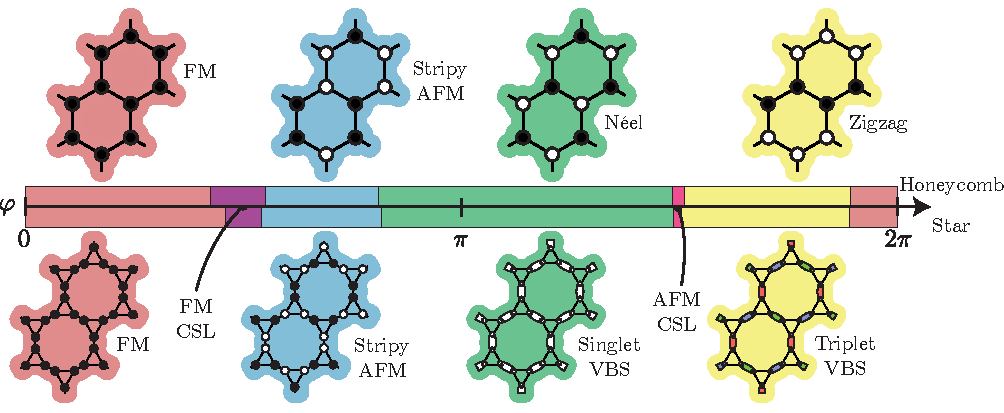
\includegraphics{kitaev_heisenberg_star/figures/phase_diagram.pdf}
    \caption{The Majorana fermion band structure calculated for the chiral QSL phase within a parton MFT for a strip-geometry, with periodic boundaries in the $x$-direction and open boundaries in the $y$ direction. We have tuned the model to the antiferromagnetic Kitaev regime ($\alpha = 1.45\pi$) in the vicinity of the soluble point. Energies are plotted as a function of momentum in the $y$-direction, for a sample with $L_x = L_y = 200$. The Chern number $\nu$ of the three bands is labelled. States are coloured according to their inverse participation ratio, where red indicates a localised edge mode and grey a delocalised bulk mode.}
    \label{fig:lattice_and_phase_diagram}
\end{figure}

We briefly recap the phase diagram of the standard Kitaev model on the honeycomb lattice~\cite{chaloupka_zigzag_2013, gohlke_dynamics_2017}, which will be useful for elucidating the novel features of the star lattice. The full phase diagram in $\varphi$ contains the two Kitaev spin liquid phases, and four distinct magnetically ordered phases. These come in two pairs, where the two phases in each pair can be mapped exactly onto one another by rotating the coordinate system of certain spins in the lattice~\cite{schaffer_quantum_2012, chaloupka_kitaev-heisenberg_2010} according to a four unit cell pattern. 
%
Around $\varphi = 0$ ($K, J >0$) the system orders into a ferromagnetic (FM) phase, with completely aligned spins. Around $\varphi = 0.6\pi$ ($K>0, J<0$) the system forms a stripy ordered phase, which can be mapped onto the ferromagnetic phase by the four unit cell spin rotation. Around $\varphi = \pi$ ($K,J < 0$) the system forms an antiferromagnetic (AFM) N\'eel ordered phase, which is again isomorphic to a zigzag phase that appears around $\varphi = 1.6\pi$ ($K<0, J>0$). The mapping implies that the dynamics in each pair of isomorphic phases is identical.

Next, let us turn our attention to the star lattice, We numerically determine the ground state across the full range of $\varphi$ using the density matrix renormalisation group (DMRG) method. DMRG is a variational optimisation algorithm used to find the ground state of many-body Hamiltonians. Although it is predominantly used for characterising 1D physics, recent work has shown that it can provide an effective description of several 2D frustrated systems~\cite{gohlke_dynamics_2017,shinjo_density-matrix_2015}. Here, we construct the Hamiltonian on a system with infinite cylindrical geometry, with two unit cells (12 sites) spanning the finite circumference. The ground state is represented with a matrix product state ansatz with bond dimension $\chi = 1600$, and is calculated using the TeNPy library~\cite{tenpy} for 1000 values of $\varphi$ across the full range $[0,2\pi]$.


\begin{figure*}[t]
    \centering
    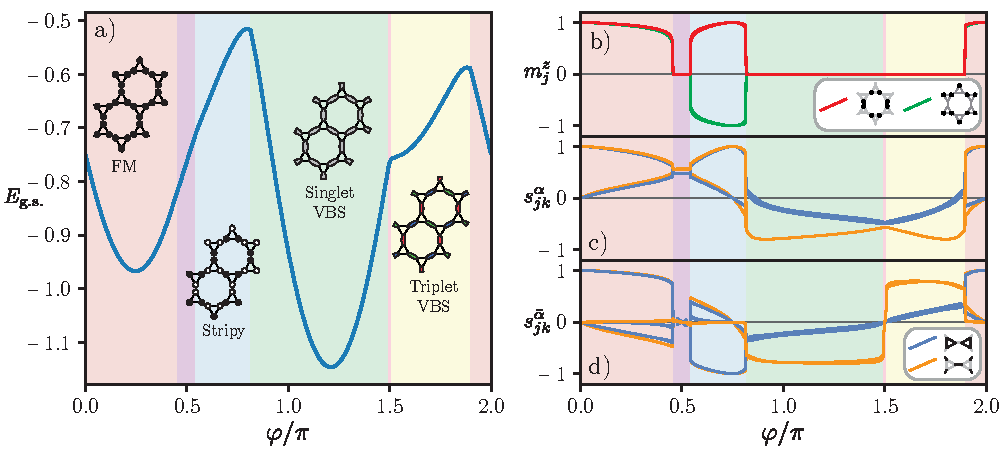
\includegraphics[width = \textwidth]{kitaev_heisenberg_star/figures/dmrg_evidence.pdf}
    \caption { 
    Full iDMRG results for the star lattice KH model as a function of the parameter $\varphi$, defined in eqn.~\ref{eqn:phi_def}. Phase boundaries are indicated with background colour.
    \textbf{a)} Ground state energy per site as a function of $\varphi$.  The four non-KSL phases are shown with a diagram of the corresponding phase. KSL phases appear at $\varphi = 0.5\pi, 1.5\pi$.
    \textbf{b)} Expectation $z$-component of magnetisation for each site on the lattice $m_z = \braket{\sigma_j^z}$.
    \textbf{c)} Spin-spin correlations for each bond in the \textit{on-colouring} direction, $\braket{\sigma_j^\alpha \sigma_k^\alpha}$.
    \textbf{d} Spin-spin correlations for each bond in the two remaining \textit{off-colouring} directions, $\braket{\sigma_j^\alpha \sigma_k^\alpha}$.  In (c) and (d), correlations for in-triangle bonds are coloured in blue, whereas inter-triangle bonds are shown in orange.  
    }
    \label{fig:dmrg_results}
\end{figure*}
%In the Kitaev phase, we expect to encounter substantial finite size effects on such a small lattice, and the system will generally order into a flux configuration other than the ground state flux sector given in~\cite{Yao_2007, Cassella_2023}. This flux sector will have lower energy than the ground state, so we expect that the phase boundaries determined will correspond to a slightly more stable Kitaev phase than in the true thermodynamic limit. 

Using this method, we find that the phase diagram contains six distinct phases, shown in Fig.~\ref{fig:lattice_and_phase_diagram}b. In the regime where $K>0$ ($\varphi \sim [-0.2\pi, 0.8\pi]$) -- which we will refer to as the broadly FM regime -- we find two magnetically ordered phases. Around $\varphi = 0$, we encounter the standard FM phase with aligned spins, which includes the FM Heisenberg point at $\varphi = 0$. 

Around $\varphi = 0.6$ we find a stripy phase with an equal proportion of spin up and spin down sites. This phase may be understood in direct analogy with the stripy ordered phase found in the honeycomb model, where each triangle in the star lattice can be treated as an effective spin half site, since they form either a $\ket{\uparrow_{\textup{eff}}} = \ket{\uparrow \uparrow \downarrow}$ or a $\ket{\downarrow_{\textup{eff}}} = \ket{\uparrow \downarrow \downarrow}$ state. These effective spin half triangles then order identically to the stripe order found on the honeycomb. Remarkably, we also find that the FM and stripy ground states can be mapped onto  one under an extended four unit cell rotation described in \textsection\ref{sec:spin_flip_transformation}.
% Around $\varphi = 0.5\pi$ the system forms a ferromagnetic CSL consistent with the exact solution of~\cite{Yao_2007}. 

In the regime where $K<0$ ($\varphi \sim [0.8\pi, 1.8\pi]$) -- referred to as the broadly AFM regime -- the system forms two distinct VBS phases. Around $\varphi = \pi$ we have a singlet VBS, where the states form spin singlets
\begin{align}
    \ket{s} = \frac{1}{\sqrt 2} \left ( \ket{\uparrow \downarrow}-\ket{ \downarrow \uparrow} \right ), \label{eqn:s_def}
\end{align}
on the inter-triangle bonds. At the point $\varphi = \pi$ the system is exactly an antiferromagnetic Heisenberg model, where previous studies support our conclusions \cite{richter_absence_2004, yang_competing_2010, jahromi_infinite_2018}. This VBS phase has no analogue on the honeycomb lattice, which forms a N\'eel ordered ground state. This is due to geometric frustration, where the presence of odd cycles on the star lattice disallows the formation of the N\'eel AFM phase. 

Around $\varphi = 1.7\pi$, the system forms an exotic spin triplet VBS. Here the spins on each bond form one of three triplet phases depending on the bond type. Bonds of type $x, y$ or $z$ form a $\ket{t_x}$, $\ket{t_y}$ or $\ket{t_z}$ state respectively, defined as
\begin{align}
    \ket{t_x} = \frac{i}{\sqrt 2} \left ( \ket{\uparrow \uparrow}-\ket{\downarrow \downarrow} \right ), \label{eqn:tx_def} \\
    \ket{t_y} = \frac{1}{\sqrt 2} \left ( \ket{\uparrow \uparrow}+\ket{\downarrow \downarrow} \right ),\label{eqn:ty_def} \\
    \ket{t_z} =  \frac{-i}{\sqrt 2} \left ( \ket{\uparrow \downarrow}+\ket{\downarrow \uparrow} \right ).\label{eqn:tz_def}
\end{align}
We will show below in in \textsection\ref{sec:spin_flip_transformation} that the singlet and triplet VBS phases are isomorphic under a generalized four unit cell spin rotation.

Around $\varphi \sim 0.5\pi$ and $\varphi \sim 1.5\pi$ the system forms two extended chiral spin liquid phases. We notes that the AFM Kitaev phase is stable over a much smaller region of phase space than the FM QSL. This can be explained by noticing that the two competing phases (both the VBS phases) have lower energy than their ferromagnetic counterparts, whereas the energy scale of both Kitaev phases are identical. Thus, as we tune across the phase diagram, the VBS phases very quickly become energetically favourable over the QSL.

As in the honeycomb case, all phase transitions corresponded to cusps in the ground state energy, indicating that the transitions are first order. However, it remains an open and numerically challenging question whether they remain first order in the thermodynamic limit. Full iDMRG results are discussed in Appendix~\ref{apx:DMRG_results}. 

Finally, we have confirmed that the pure Kitaev points ($\varphi = 0.5\pi$ or $1.5\pi$) exactly recover the chiral QSL studied Yao and Kivelson~\cite{yao_exact_2007}. Here, the model is exactly solvable and can be decoupled into non-interacting Majorana fermions in the presence of a static $\mathbb Z_2$ gauge field~\cite{kitaev_anyons_2006}. However, as soon as we tune away from these points (and some Heisenberg interactions are present) the $\mathbb Z_2$ gauge field is no longer conserved and the system ceases to be exactly solvable. In Appendix \ref{sec:mft}, we study the entire phase diagram using a Majorana MFT. As shown in Fig.~\ref{fig:lattice_and_phase_diagram}b we recover the DMRG phase diagram qualitatively but, as common for parton MFT, we find an enhancement of the region of stability of the QSL regimes.  
One additional advantage of the Majorana MFT is that we can obtain the excitation spectrum of the chiral QSLs away from the soluble points as. In Fig.~\ref{fig:kitaev_chern_bands} we show the Majorana band structure on a cylinder geometry with open boundary conditions. The nonzero Chern numbers of the bulk bands give rise to chiral edge modes (indicated in red), whose dispersion are weakly renormalized by the presence of Heisenberg interactions. 

\section{Isometries of the Kitaev-Heisenberg Phase Diagram}\label{sec:spin_flip_transformation}
\begin{figure}[t]
    \centering
    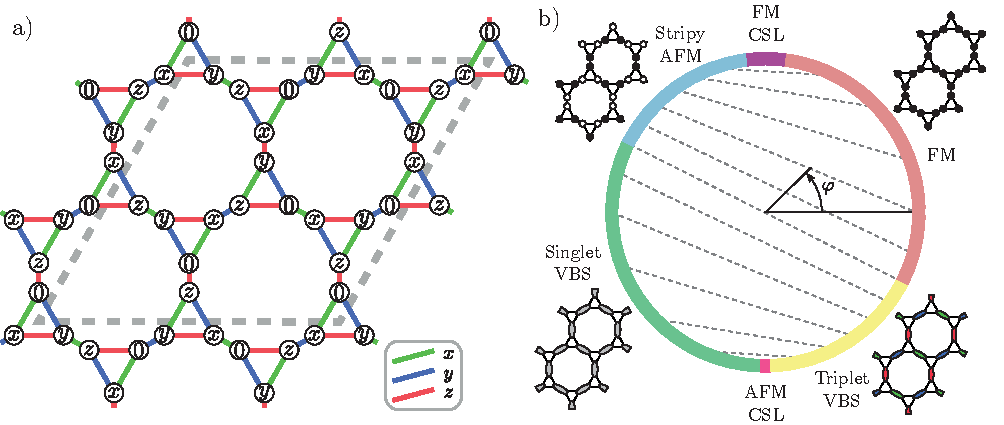
\includegraphics[]{kitaev_heisenberg_star/figures/transformation.pdf}
    \caption{
    \textbf{a)} Plot of the four unit cell transformation that encodes the isometry of the KH phase diagram. Each $0$-marked site is untouched, however the sites labelled with $x$, $y$ or $z$ each experience a $\pi$-rotation around the labelled axis in spin space. Bond-types are indicated by colour. Enlarged unit cell is depicted with the dashed rhombus. \textbf{b)} The KH phase diagram as parametrised by $\varphi$ defined in Eqn.~\ref{eqn:phi_def}. Dashed lines indicate points that are isomorphic under the spin rotation. 
    }
    \label{fig:spin_transformation}
\end{figure}

One of the remarkable aspects of the Heisenberg-Kitaev model on the honeycomb lattice is a hidden symmetry between different phases of the model~\cite{chaloupka_zigzag_2013}. In this section we show that similar relations hold on the star lattice, which help to understand the phase diagram and clarify the connection between the distinct types of VBS phases. 

Let us introduce a spin transformation by dividing the spins in the system into four sets, each labelled with $0$, $x$, $y$ or $z$, arranged in a four-unit-cell pattern as shown in Fig.~\ref{fig:Appendix_transformation}a. Spins marked with $0$ will be left untouched, however on the other spins we apply a $\pi$-rotation in spin space, where the axis of rotation is determined by the site labels. Under such a rotation, the sign of the two spin operators that do not line up with the rotational axis will be flipped, for example if the site $j$ is labelled with $x$ we have
\begin{align}
    \begin{aligned}
        \sigma_j^x &\rightarrow \sigma_j^x \\
        \sigma_j^y &\rightarrow -\sigma_j^y \\
        \sigma_j^z &\rightarrow -\sigma_j^z,
    \end{aligned}
\end{align}
with a similar relation for $y$ and $z$-labelled sites.

Under this transformation, we note that every $x$-bond is always bordered by either a $0 - x$ pair of sites or a $y-z$ pair. Thus, every $x$-type bond operator in $H$ transforms according to
\begin{align}
    \begin{aligned}
        \sigma_j^x\sigma_k^x &\rightarrow \sigma_j^x\sigma_k^x \\
        \sigma_j^y\sigma_k^y &\rightarrow -\sigma_j^y\sigma_k^y \\
        \sigma_j^z\sigma_k^y &\rightarrow -\sigma_j^z\sigma_k^y.
    \end{aligned}
\end{align}
Similarly, $y$-bonds are bordered by $0-y$ or $x-z$, and $z$-bonds are bordered by $0-z$ or $x-y$. These both transform analogously under the spin rotation, where the on-colouring direction remains unchanged and the off-colouring directions have their sign flipped. Thus, our spin rotation is equivalent to transforming the parameters of the Hamiltonian according to
\begin{align}
    K \rightarrow K,\ J \rightarrow -J.
\end{align}
In terms of the single parameter $\varphi$, this is equivalent to transforming to a new $\tilde \varphi$ that satisfies
\begin{align}
     \tan \tilde \varphi = -\tan \varphi - 1
\end{align}
with the correspondence indicated with dashed lines in Fig.~\ref{fig:Appendix_transformation}b.

Thus, we see that there is a correspondence between the ferromagnetic Hamiltonian and the stripy ordered Hamiltonian, as well as a correspondence between the singlet VBS and the stripy VBS Hamiltonians. We can similarly verify that the transformation gives the correct relation between the phases: 
First, The FM case is easy -- starting with a FM alignment in the $z$-direction, we can see that any site labelled with $x$ or $y$ has its spin flipped, which leads precisely to the stripy magnetically ordered phase. Second, the we look at the more subtle VBS correspondence. A spin singlet on an $x$-labelled bond will be adjacent to either a $0-x$ pair of sites, in which case the resulting state will be transformed as
\begin{align}
    \ket s  \sim 
    \ket{\uparrow \downarrow} - \ket{\downarrow \uparrow} 
    \rightarrow 
    \ket{\uparrow \uparrow} - \ket{\downarrow \downarrow} 
    \sim \ket{t_x},
\end{align}
or the bond will border two sites of type $y-z$, in which case the transformation is
\begin{align}
    \ket s  \sim 
    \ket{\uparrow \downarrow} - \ket{\downarrow \uparrow} 
    \rightarrow 
    i \ket{\downarrow \downarrow} - i \ket{\uparrow \uparrow} 
    \sim \ket{t_x}.
\end{align}
In both cases we see that (up to a phase) the singlet is mapped onto a triplet $\ket{t_x}$ state. Similar arguments apply for $y$- and $z$-bonds. Thus, from the mapping we observe that the resulting stripy VBS consists of a condensate of triplet states, where each $x$-bond has a $\ket{t_x}$ triplet, each $y$-bond has a $\ket{t_y}$ triplet and so on. This is perfectly consistent with our results in section \ref{sec:dmrg} and the Appendix \ref{sec:mft}. 
